\let\negmedspace\undefined
\let\negthickspace\undefined
\documentclass[journal]{IEEEtran}
\usepackage[a5paper, margin=10mm, onecolumn]{geometry}
%\usepackage{lmodern} % Ensure lmodern is loaded for pdflatex
% \usepackage{tfrupee} % Include tfrupee package

\setlength{\headheight}{1cm} % Set the height of the header box
\setlength{\headsep}{0mm}     % Set the distance between the header box and the top of the text

\usepackage{gvv-book}
\usepackage{gvv}
\usepackage{cite}
\usepackage{amsmath,amssymb,amsfonts,amsthm}
\usepackage{algorithm}
\usepackage{algorithmic}
\usepackage{graphicx}
\usepackage{textcomp}
\usepackage{xcolor}
\usepackage{txfonts}
\usepackage{listings}
\usepackage{enumitem}
\usepackage{mathtools}
\usepackage{gensymb}
\usepackage{comment}
\usepackage[breaklinks=true]{hyperref}
\usepackage{tkz-euclide} 
\usepackage{listings}
% \usepackage{gvv}                                        
\def\inputGnumericTable{}                                 
\usepackage[latin1]{inputenc}                                
\usepackage{color}                                            
\usepackage{array}                                            
\usepackage{longtable}                                       
\usepackage{calc}                                             
\usepackage{multirow}                                         
\usepackage{hhline}                                           
\usepackage{ifthen}                                           
\usepackage{lscape}
% \usepackage{algpseudocode}
\begin{document}

\bibliographystyle{IEEEtran}
\vspace{3cm}

\title{NCERT 10.4.3.6}
\author{EE24BTECH11053 - S A Aravind Eswar}
% \maketitle
% \newpage
% \bigskip
{\let\newpage\relax\maketitle}

\renewcommand{\thefigure}{\theenumi}
\renewcommand{\thetable}{\theenumi}
\setlength{\intextsep}{10pt} % Space between text and floats

\textbf{Question:} The diagonal of a rectangular field is 60 metres more than the shorter side. If the longer side is 30 metres more than the shorter side, find the sides of the field.

\subsection{Theoretical Method: }
    Let,

    longer side = $l$

    shorter side = $b$

    Given,
    \begin{align}
        \sqrt{l^2 + b^2} = b + 60\\
        l = b+30 
    \end{align}

    Substituting,
    \begin{align}
        b^2 - 60b - 2700 = 0
    \end{align}
    Solving,
    \begin{align}
        b = 90\\
        b = -30
    \end{align}
    
    But as length cannot be negative,
    \begin{align}
        b = 90
    \end{align}
    From this,
    \begin{align}
        l = 120
    \end{align}
\subsection{Fixed Point iterations: }
    The most primitive method to calculate roots,
    Given,
    \begin{align}
        x^2 - 60\,x - 2700 = 0
    \end{align}
    Rearranging, we get,
    \begin{align}
        x &= \frac{2700}{x} + 60\\
        x &= g(x)
    \end{align}

    Now applying Fixed point iteration, $x_{n+1} = g(x_n)$, we get,
    \begin{align}
        x_{n+1} = \frac{2700}{x_n} + 60
    \end{align}
    Taking inital guess as 150, we get,
    \begin{align}
        x_{n} = 89.99999999957511
    \end{align}
    Tolerance = 10e-10\\
    Number of iterations = 23


\subsection{Newton's iterations: }
    The equation for Newton-Raphson Method is given by,
    \begin{align}
        x_{n+1} = x_n - \frac{f(x_n)}{f^\prime(x_n)}
    \end{align}
    Given,
    \begin{align}
        f(x_n) = x_n^2 - 60\,x_n - 2700\\
        f^\prime(x_n) = 2\,x_n - 60
    \end{align}
    We get,
    \begin{align}
        x_{n+1} = x_n - \frac{x_n^2 - 60\,x_n - 2700}{2\,x_n - 60}
    \end{align}

    Taking inital guess,
    \begin{align}
        x_0 = 150
    \end{align}

    We get,
    \begin{align}
        x_n = 90.00000000000007
    \end{align}
    Tolerance = 10e-10\\
    Number of iterations = 5
\subsection{Secant Method: }
    Even though Newton's Method will suffice in this case, it has a few drawbacks. To fix them, we will also look at Secant Method.

    We will need 2 inital guesses for this method.

    The equationn for Secant method is given by,

    \begin{align}
        x_{n+1} = x_n - \frac{f(x_n)(x_n - x_{n-1})}{f(x_{n})-f(x_{n-1})}
    \end{align}
    Substituting,
    \begin{align}
        x_{n+1} = x_n - \frac{\brak{x_n^2 - 60\,x_n - 2700}\brak{x_n - x_{n-1}}}{\brak{x_n^2 - 60\,x_n - 2700} - \brak{x_{n-1}^2 - 60\,x_{n-1} - 2700}}
    \end{align}

    Taking inital guesses as,
    \begin{align}
        x_0 = 150\\
        x_1 = 50
    \end{align}
    We get,
    \begin{align}
        x_n = 90.0
    \end{align}
    Tolerance = 10e-10\\
    Number of iterations = 7

\subsection{Matrix Method}
We also have a method to solve it without any iterations with the help of companion matrix.

If the given polynomial is,
\begin{align}
	P(x) = c_0 + c_1\,x + c_2\,x^2 + \dots + c_{n-1}\,x^{n-1} + x^n
\end{align}

Then the companion matrix is given as,

\begin{align}
	M = \myvec{0 & 0 & \dots & 0 & -c_0\\1 & 0 & \dots & 0 & -c_1\\0 & 1 & \dots & 0 & -c_2\\\vdots & \vdots & \vdots & \vdots &\vdots \\0 & 0 & \dots & 1 & -c_{n-1}}
\end{align}

For our equation,
\begin{align}
    P(x) = -2700 - 60\,x + x^2
\end{align}

The companion matrix is given as,
\begin{align}
    M = \myvec{0 & 2700\\1 & 60}
\end{align}

We can find the eigenvalues using QR algorithm.

\begin{align}
    M_n = Q_n\,R_n\\
    M_{n+1} = R_n\,Q_n
\end{align}

The diagonal elements of $M_n$ after enough iterations will give you the eigenvalues.

The eigenvalues of the above matrix are,
\begin{align}
    \lambda_1 = 90\\
    \lambda_2 = -30
\end{align}

As the root cannot be negative,
\begin{align}
    x = 90
\end{align}


    \begin{figure}[ht]  
        \centering  
        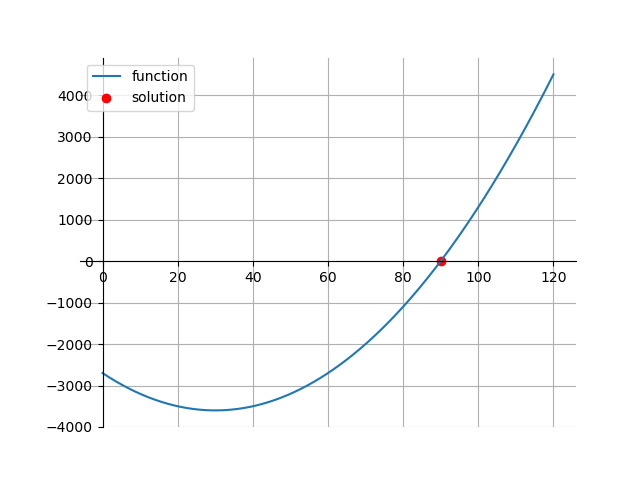
\includegraphics[width=\columnwidth]{figs/fig1.png}  
        \caption{Verification}
        % \columnwidth
    \end{figure}

\end{document}
